\documentclass[
11pt, % The default document font size, options: 10pt, 11pt, 12pt
%codirector, % Uncomment to add a codirector to the title page
]{charter} 




% El títulos de la memoria, se usa en la carátula y se puede usar el cualquier lugar del documento con el comando \ttitle
\titulo{Sistema de control y monitoreo de tiempo de abastecimiento de camiones basado en una OrangePI5} 

% Nombre del posgrado, se usa en la carátula y se puede usar el cualquier lugar del documento con el comando \degreename
\posgrado{Carrera de Especialización en Sistemas Embebidos} 
%\posgrado{Carrera de Especialización en Internet de las Cosas} 
%\posgrado{Carrera de Especialización en Intelegencia Artificial}
%\posgrado{Maestría en Sistemas Embebidos} 
%\posgrado{Maestría en Internet de las cosas}

% Tu nombre, se puede usar el cualquier lugar del documento con el comando \authorname
\autor{Anthony Martyn Maisincho Jivaja} 

% El nombre del director y co-director, se puede usar el cualquier lugar del documento con el comando \supname y \cosupname y \pertesupname y \pertecosupname
\director{MSc. Jefferson Cunalata}
\pertenenciaDirector{SIEMAV S.A} 
% FIXME:NO IMPLEMENTADO EL CODIRECTOR ni su pertenencia
\codirector{John Doe} % para que aparezca en la portada se debe descomentar la opción codirector en el documentclass
\pertenenciaCoDirector{FIUBA}

% Nombre del cliente, quien va a aprobar los resultados del proyecto, se puede usar con el comando \clientename y \empclientename
\cliente{MSc. Geovanny Arguello}
\empresaCliente{SIEMAV S.A}

% Nombre y pertenencia de los jurados, se pueden usar el cualquier lugar del documento con el comando \jurunoname, \jurdosname y \jurtresname y \perteunoname, \pertedosname y \pertetresname.
\juradoUno{Nombre y Apellido (1)}
\pertenenciaJurUno{pertenencia (1)} 
\juradoDos{Nombre y Apellido (2)}
\pertenenciaJurDos{pertenencia (2)}
\juradoTres{Nombre y Apellido (3)}
\pertenenciaJurTres{pertenencia (3)}
 
\fechaINICIO{22 de agosto de 2023}		%Fecha de inicio de la cursada de GdP \fechaInicioName
\fechaFINALPlan{10 de octubre de 2023} 	%Fecha de final de cursada de GdP
\fechaFINALTrabajo{15 de mayo de 2024}	%Fecha de defensa pública del trabajo final


\begin{document}

\maketitle
\thispagestyle{empty}
\pagebreak


\thispagestyle{empty}
{\setlength{\parskip}{0pt}
\tableofcontents{}
}
\pagebreak


\section*{Registros de cambios}
\label{sec:registro}


\begin{table}[ht]
\label{tab:registro}
\centering
\begin{tabularx}{\linewidth}{@{}|c|X|c|@{}}
\hline
\rowcolor[HTML]{C0C0C0} 
Revisión & \multicolumn{1}{c|}{\cellcolor[HTML]{C0C0C0}Detalles de los cambios realizados} & Fecha      \\ \hline
0      & Creación del documento                                 &\fechaInicioName \\ \hline
1.0    & Se completa hasta el punto 5                           & 07/09/2023 \\ \hline
2.0    & Se completa hasta el punto 9 y se hacen correciones    & 14/09/2023 \\ \hline
%		  Se puede agregar algo más \newline
%		  En distintas líneas \newline
%		  Así                                                    & dd/mm/aaaa \\ \hline
%3      & Se completa hasta el punto 11 inclusive                & dd/mm/aaaa \\ \hline
%4      & Se completa el plan	                                 & dd/mm/aaaa \\ \hline
\end{tabularx}
\end{table}

\pagebreak



\section*{Acta de constitución del proyecto}
\label{sec:acta}

\begin{flushright}
Guayaquil, \fechaInicioName
\end{flushright}

\vspace{2cm}

Por medio de la presente se acuerda con el Ing. \authorname\hspace{1px} que su Trabajo Final de la \degreename\hspace{1px} se titulará ``\ttitle'', consistirá esencialmente en integrar en una OrangePI5 funcionalidades de un controlador lógico programable y ejecutar algoritmo de detección de objetos en videos en tiempo real, y tendrá un presupuesto preliminar estimado de 600 h de trabajo y \$10145 USD, con fecha de inicio \fechaInicioName\hspace{1px} y fecha de presentación pública \fechaFinalName.

Se adjunta a esta acta la planificación inicial.

\vfill

% Esta parte se construye sola con la información que hayan cargado en el preámbulo del documento y no debe modificarla
\begin{table}[ht]
\centering
\begin{tabular}{ccc}
\begin{tabular}[c]{@{}c@{}}Dr. Ing. Ariel Lutenberg \\ Director posgrado FIUBA\end{tabular} & \hspace{2cm} & \begin{tabular}[c]{@{}c@{}}\clientename \\ \empclientename \end{tabular} \vspace{2.5cm} \\ 
\multicolumn{3}{c}{\begin{tabular}[c]{@{}c@{}} \supname \\ Director del Trabajo Final\end{tabular}} \vspace{2.5cm} \\
%\begin{tabular}[c]{@{}c@{}}\jurunoname \\ Jurado del Trabajo Final\end{tabular}     &  & \begin{tabular}[c]{@{}c@{}}\jurdosname\\ Jurado del Trabajo Final\end{tabular}  \vspace{2.5cm}  \\
%\multicolumn{3}{c}{\begin{tabular}[c]{@{}c@{}} \jurtresname\\ Jurado del Trabajo Final\end{tabular}} \vspace{.5cm}                                                                     
\end{tabular}
\end{table}




\section{1. Descripción técnica-conceptual del proyecto a realizar}
\label{sec:descripcion}

SIEMAV S.A, se dedica a generar soluciones tecnológicas innovadoras mediante el desarrollo de hardware y software a medida con el objetivo de mejorar la competitividad de sus clientes y optimizar su productividad. Actualmente uno de sus clientes requiere mejorar los tiempos de abastecimiento de camiones en uno de sus centros de distribución. 

SIEMAV S.A propuso un sistema basado en un controlador lógico programable (PLC) y una mini CPU de altas prestaciones. El PLC, actualmente se encarga del control del tablero eléctrico, mientras que la CPU es empleada para ejecutar el algoritmo de detección de objetos en imágenes y videos en tiempo real.

Siempre buscando optimizar recursos y abaratar costos al producto final, se planteó utilizar un sistema embebido que sea capaz de asumir el rol del PLC y la CPU. Para esto se debe reestructurar el proyecto e integrar todo el sistema en una ORANGEPI5. Actualmente, este SBC (\textit{System board Computer}) no ha sido utilizado en la empresa. Por lo tanto, se tiene como desafío migrar toda la funcionalidad del sistema en una sola placa embebida. 

Utilizar una sola placa embebida como la ORANGEPI5 es una solución altamente eficiente y coste-efectiva. Al integrar todas las funcionalidades en este equipo se disminuirá la complejidad de la infraestructura. Además,  se aprovechará su unidad de procesamiento de redes neuronales para la detección de los camiones parqueados y también sus periféricos para el control del tablero. Esta integración permitirá  una mayor eficiencia energética, ahorro en términos de hardware, espacio físico, mantenimiento y optimización de recursos. 

En la Figura \ref{fig:diagBloques} se presenta el diagrama en bloques del sistema. Se identifican tres fases, la primera es el montaje del algoritmo YOLOV8. La segunda es la comunicación y el manejo de la placa PLC SIEMAV, que permitirá controlar el tablero eléctrico. Finalmente, comunicación con cámaras IP y tablero LED, importante para la obtención de datos de imágenes e interfaz visual para los operadores, respectivamente.
\begin{figure}[htpb]
\centering 
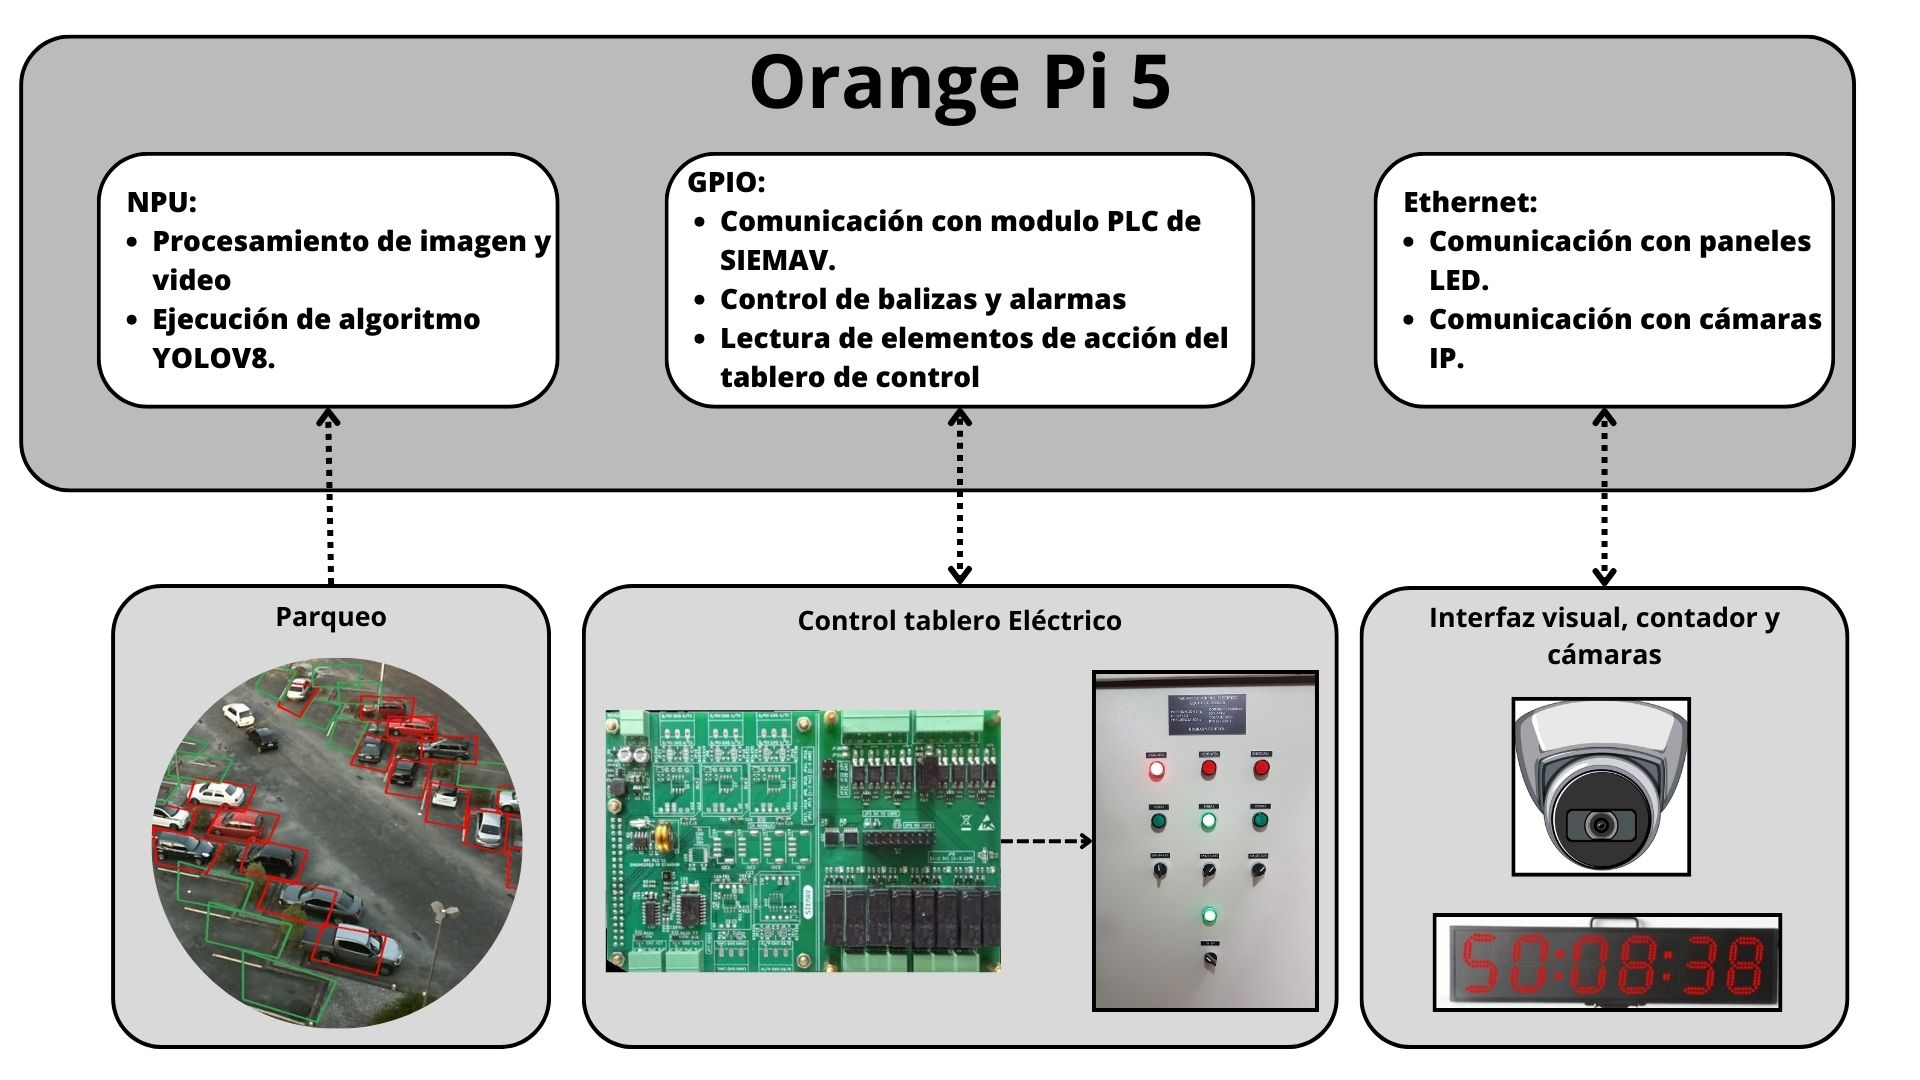
\includegraphics[width=1\textwidth]{./Figuras/diagramabloques.jpg}
\caption{Diagrama en bloques del sistema}
\label{fig:diagBloques}
\end{figure}

\vspace{25px}


\section{2. Identificación y análisis de los interesados}
\label{sec:interesados}

\begin{table}[ht]
%\caption{Identificación de los interesados}
%\label{tab:interesados}
\begin{tabularx}{\linewidth}{@{}|l|X|X|l|@{}}
\hline
\rowcolor[HTML]{C0C0C0} 
Rol           & Nombre y Apellido & Organización 	& Puesto 	\\ \hline
Auspiciante   & -                 &   SIEMAV S.A    &-         	\\ \hline
Cliente       & \clientename      &\empclientename	& C.T.O       	\\ \hline
Responsable   & \authorname       & FIUBA        	& Alumno 	\\ \hline
Colaboradores &Ing. Alexis Mora& SIEMAV S.A      & Consultor firmware\\ \hline
Orientador    & \supname	      & \pertesupname 	& Director Trabajo final \\ \hline
\end{tabularx}
\end{table}

\begin{itemize}
	\item Auspiciante: SIEMAV S.A que impulsa el desarrollo tecnológico, un gran apoyo en adquisición de todos los equipos necesarios.
	\item Equipo: Alexis Mora, jefe de investigación y desarrollo, experto en miniordenadores como la OrangePI5 y con buen criterio al momento de desarrollar proyectos.
	\item Orientador: con amplia trayectoria en el desarrollo de hardware y firmware para sistemas embebidos, ayudará mucho con soporte, consultoría y objetivos del proyecto.
\end{itemize}


\section{3. Propósito del proyecto}
\label{sec:proposito}
El propósito del proyecto es integrar todo el sistema de control y monitoreo de tiempo de abastecimiento de camiones en un solo sistema embebido. Con esto se quiere lograr un sistema más económico, reducir la complejidad de la infraestructura y aprovechar al máximo la OrangePI5.

\section{4. Alcance del proyecto}
\label{sec:alcance}
Las actividades dentro del alcance del proyecto consiste en lo siguiente:
\begin{itemize}
	\item Estudio de la tarjeta PLC de la empresa auspiciante.
	\item Adaptación y correciones del hardware actual de la tarjeta PLC para que funcione con la OrangePI5. 
	\item Desarrollo de software para manejo de la tarjeta PLC de SIEMAV y pruebas de su funcionamiento.
	\item Desarrollo de software para el manejo del tablero LED.
	\item Estudio de como usar la NPU de la OrangePI5.
	\item Integrar algoritmo de detección de objetos e imágenes YOLOV8 en la ORANGEPI5 usando la NPU.
	\item Estudio de como integrar diferentes tareas en una ORANGEPI5, ya que se debe interactuar con la tarjeta PLC, extraer imágenes y procesarlas y comunicarse con tableros LED.
\end{itemize}
Las actividades fuera del alcance del proyecto son las siguientes:
\begin{itemize}
	\item Entrenamiento del algoritmo de detección de imágenes.
	\item Correcciones a características de funcionamiento del algoritmo YOLOV8.
	\item Implementación del tablero de control eléctrico.
	\item Instalación en campo del sistema.
\end{itemize}

\section{5. Supuestos del proyecto}
\label{sec:supuestos}


Para el desarrollo del presente proyecto se supone que:

\begin{itemize}
	\item La importación de la ORANGEPI5 no tomará más de un mes.
	\item Correr el algoritmo de detección de objetos e imágenes en la OrangePI5 no implicará profundizar en este tema.
	\item Se dispondrá de todos los recursos necesarios para el desarrollo eficiente del proyecto.
	\item La versión actual de la tarjeta "Módulo PLC"  de SIEMAV, no requerirá de extensas modificaciones para la adaptación a la OrangePI5.
	\item Tomará menos de tres meses disponer del nuevo "Módulo PLC".
	\item Habrá un seguimiento por parte del director y del colaborador del proyecto al menos una vez mensualmente.
\end{itemize}


\section{6. Requerimientos}
\label{sec:requerimientos}

\begin{enumerate}
	\item Requerimientos funcionales
		\begin{enumerate}
			\item El sistema debe reconocer cuando un camión de abastecimiento se encuentra parqueado.
			\item El sistema debe registrar el tiempo que se tomó durante el abastecimiento.
			\item El usuario debe poder visualizar el número de andén y el tiempo transcurrido durante el abastecimiento.
			\item El usuario reconocerá el estado del sistema visualizando las balizas.
			\item El sistema debe tener dos modos de funcionamiento, manual y automático.
			\item El usuario debe poder operar el sistema en modo manual mediante un tablero de control.
		\end{enumerate}
	\item Requerimientos del controlador del tablero eléctrico
		\begin{enumerate}
			\item La OrangePI5 debe leer estado de selectores, pulsadores, contactos auxiliares y paro de emergencia.
			\item La OrangePI5 controlará las balizas mediante el manejo de las salidas de la tarjeta PLC de SIEMAV.
			\item La OrangePI5 controlará las luces pilotos verde y rojo mendiante la tarjeta PLC de SIEMAV.
			\item Dentro del tablero se tendrá la OrangePI5 como tarjeta maestro o controladora del sistema.
		\end{enumerate}
	\item Requerimiento de interfaz de usuario
		\begin{enumerate}
			\item El tablero mediante sus luces pilotos verde y rojo por andén, indicarán el estado de inicio y final del proceso.
			\item Un selector de tres posiciones seleccionará el modo de funcionamiento del tablero, ya sea manual o automático.
			\item Se contará con un pulsador por andén, el cual deberá ser presionado para iniciar el proceso y conteo del temporizador.
			\item Cada andén tendrá una baliza, el color verde indica que hay tiempo y el rojo que se expiró el tiempo.
			\item Se utilizará tableros LED como cronómetros digitales, donde el usuario tendrá información del tiempo actual.
		\end{enumerate}
	\item Requerimientos de software
		\begin{enumerate}
			\item El software debe detectar cuando un andén es ocupado por el camión, tomando la hora y registrarla como hora de entrada.
			\item Cuando el camión desocupe el andén, se registra la hora de salida.
			\item La creación de la API que controlará la tarjeta PLC de SIEMAV, será desarrollado en python.
			\item Se desarrollará una API en python para controlar los tableros de LED.
			\item Se debe utilizar la NPU de la OrangePI5 para el procesamiento de imágenes y vídeos.
		\end{enumerate}
	\item Requerimientos de diseño
		\begin{enumerate}
			\item El SBC a utilizar será la OrangePI5.
		\end{enumerate}
\end{enumerate}

\section{7. Historias de usuarios (\textit{Product backlog})}
\label{sec:backlog}
Las historias de usuario llevarán un puntaje según 3 aspectos:
\begin{itemize}
	\item Dificultad: Cantidad de trabajo a realizar.
	\item Complejidad: Nivel de sofisticación del trabajo.
	\item Incertidumbre: Nivel de riesgo que involucra realizar la tarea.
\end{itemize}

\begin{enumerate}
	\item Como gerente tecnológico, deseo aprovechar al máximo la OrangePI5, de tal forma que pueda ser el CPU y PLC del proceso.
		\begin{itemize}
			\item Dificultad: 3
			\item Complejidad: 5
			\item Incertidumbre: 5
			\item Total: 13
		\end{itemize}
	\item Como operador de abastecimiento, deseo tener información del tiempo transcurrido durante la maniobra.
		\begin{itemize}
			\item Dificultad: 1
			\item Complejidad: 1
			\item Incertidumbre: 1
			\item Total: 3
		\end{itemize}	
	\item Como programador del PLC de SIEMAV, deseo tener una API práctica y sencilla para manejar las entradas y salidas de la tarjeta.
		\begin{itemize}
			\item Dificultad: 5
			\item Complejidad: 3
			\item Incertidumbre: 1
			\item Total: 13 
		\end{itemize}	
	\item Como gerente tecnológico, deseo usar la NPU de la OrangePI5 para el procesamiento de imágenes y vídeos.
		\begin{itemize}
			\item Dificultad: 5
			\item Complejidad: 5
			\item Incertidumbre: 5
			\item Total: 21
		\end{itemize}
\end{enumerate}
\section{8. Entregables principales del proyecto}
\label{sec:entregables}


Los entregables del proyecto son (ejemplo):

\begin{itemize}
	\item Documentación de uso de la NPU en la OrangePI5
	\item Repositorio de Github con los códigos desarrollados para la Implementación de las API's
	\item Informe final
\end{itemize}



\section{9. Desglose del trabajo en tareas}
\label{sec:wbs}

\begin{enumerate}
\item Planificación y gestión del proyecto (115 hs)
	\begin{enumerate}
	\item Desarrollo del plan de trabajo (20 hs)
	\item Informe de avances (15 hs)
	\item Preparación de la memoria de trabajo (40 hs)
	\item Redacción de la memoria de trabajo (40 hs)
	\end{enumerate}
\item investigación preliminar (100 hs)
	\begin{enumerate}
	\item Arquitectura y periféricos de la OrangePI5 (20 hs)
	\item Uso de la NPU en la OrangePI5 (20 hs)
	\item Estudio de protocolo UDP (20 hs)
	\item Algoritmo YOLOV8 y su aplicación usando python (40 hs)
	\end{enumerate}
\item Desarrollo de firmware (65 hs)
	\begin{enumerate}
	\item Preparación del framework (5 hs)
	\item Modulo para manejo de tarjeta PLC de SIEMAV (20 hs)
	\item Creación de API para control de PLC de SIEMAV (10 hs)
	\item Modulo para control de tablero de LED basado en tramas UDP (20 hs)
	\item API para trama UDP (10 hs)
	\end{enumerate}
\item Uso de la NPU (100 hs)
	\begin{enumerate}
	\item Adaptación del algoritmo YOLOV8 a la OrangePI5 (40 hs)
	\item Testeo del algoritmo utilizando la NPU (20 hs)
	\item Pruebas de rendimiento  (20 hs)
	\item Ajustes finos (20 hs)
	\end{enumerate}
\item Inplementación del software de la aplicación (130 hs)
	\begin{enumerate}
	\item Importación de librerías y módulos creados (10 hs)
	\item Diseño conceptual de la aplicación (20 hs)
	\item Adaptación de las diferentes tareas a la aplicación  (40 hs)
	\item Operación manual de la aplicación (20 hs)
	\item Operación automático de la aplicación (20 hs)
	\item Testeo de la aplicación (20 hs)
	\end{enumerate}
\item Pruebas finales (120 hs)
	\begin{enumerate}
	\item Prueba del modo manual (20 hs)
	\item Prueba del modo automático (20 hs)
	\item Rendimiento de la OrangePI5 durante todo el proceso (40 hs)
	\item Correcciones (20 hs)
	\end{enumerate}
\end{enumerate}

Cantidad total de horas: (630 hs)





\section{10. Diagrama de Activity On Node}
\label{sec:AoN}

\begin{consigna}{red}
Armar el AoN a partir del WBS definido en la etapa anterior. 

%La figura \ref{fig:AoN} fue elaborada con el paquete latex tikz y pueden consultar la siguiente referencia \textit{online}:

%\url{https://www.overleaf.com/learn/latex/LaTeX_Graphics_using_TikZ:_A_Tutorial_for_Beginners_(Part_3)\%E2\%80\%94Creating_Flowcharts}

\end{consigna}

\begin{figure}[htpb]
\centering 
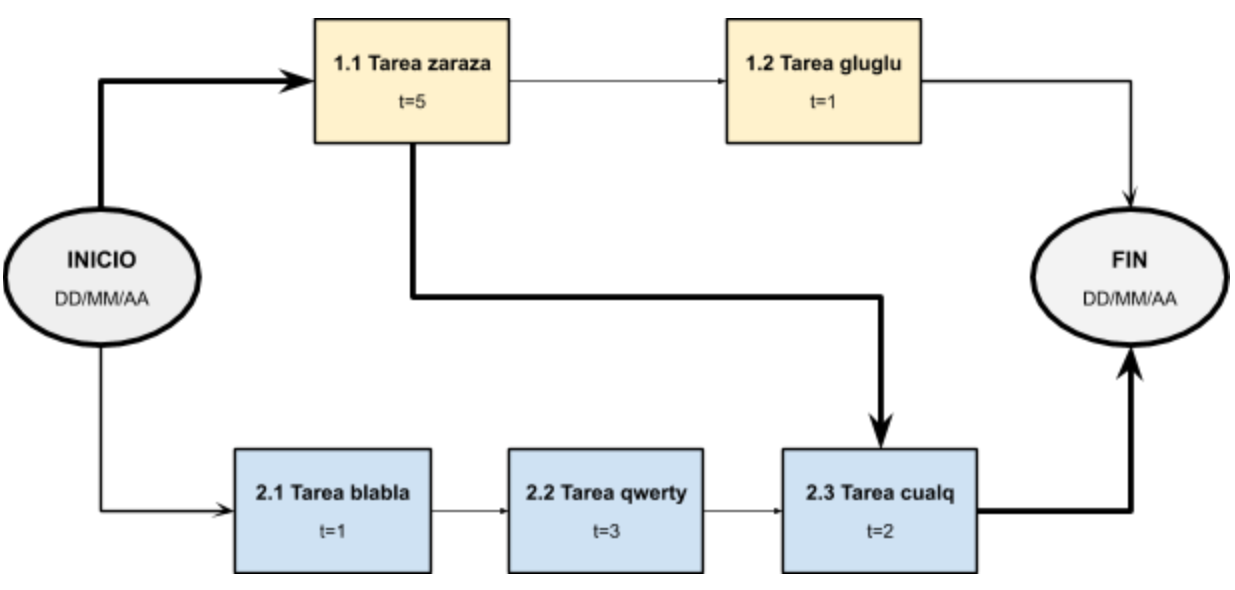
\includegraphics[width=.8\textwidth]{./Figuras/AoN.png}
\caption{Diagrama de \textit{Activity on Node}.}
\label{fig:AoN}
\end{figure}

Indicar claramente en qué unidades están expresados los tiempos.
De ser necesario indicar los caminos semicríticos y analizar sus tiempos mediante un cuadro.
Es recomendable usar colores y un cuadro indicativo describiendo qué representa cada color, como se muestra en el siguiente ejemplo:



\section{11. Diagrama de Gantt}
\label{sec:gantt}

\begin{consigna}{red}

Existen muchos programas y recursos \textit{online} para hacer diagramas de Gantt, entre los cuales destacamos:

\begin{itemize}
\item Planner
\item GanttProject
\item Trello + \textit{plugins}. En el siguiente link hay un tutorial oficial: \\ \url{https://blog.trello.com/es/diagrama-de-gantt-de-un-proyecto}
\item Creately, herramienta online colaborativa. \\\url{https://creately.com/diagram/example/ieb3p3ml/LaTeX}
\item Se puede hacer en latex con el paquete \textit{pgfgantt}\\ \url{http://ctan.dcc.uchile.cl/graphics/pgf/contrib/pgfgantt/pgfgantt.pdf}
\end{itemize}

Pegar acá una captura de pantalla del diagrama de Gantt, cuidando que la letra sea suficientemente grande como para ser legible. 
Si el diagrama queda demasiado ancho, se puede pegar primero la ``tabla'' del Gantt y luego pegar la parte del diagrama de barras del diagrama de Gantt.

Configurar el software para que en la parte de la tabla muestre los códigos del EDT (WBS).\\
Configurar el software para que al lado de cada barra muestre el nombre de cada tarea.\\
Revisar que la fecha de finalización coincida con lo indicado en el Acta Constitutiva.

En la figura \ref{fig:gantt}, se muestra un ejemplo de diagrama de Gantt realizado con el paquete de \textit{pgfgantt}. En la plantilla pueden ver el código que lo genera y usarlo de base para construir el propio.

\begin{figure}[htbp]
\begin{center}
\begin{ganttchart}{1}{12}
  \gantttitle{2020}{12} \\
  \gantttitlelist{1,...,12}{1} \\
  \ganttgroup{Group 1}{1}{7} \\
  \ganttbar{Task 1}{1}{2} \\
  \ganttlinkedbar{Task 2}{3}{7} \ganttnewline
  \ganttmilestone{Milestone o hito}{7} \ganttnewline
  \ganttbar{Final Task}{8}{12}
  \ganttlink{elem2}{elem3}
  \ganttlink{elem3}{elem4}
\end{ganttchart}
\end{center}
\caption{Diagrama de Gantt de ejemplo}
\label{fig:gantt}
\end{figure}


\begin{landscape}
\begin{figure}[htpb]
\centering 
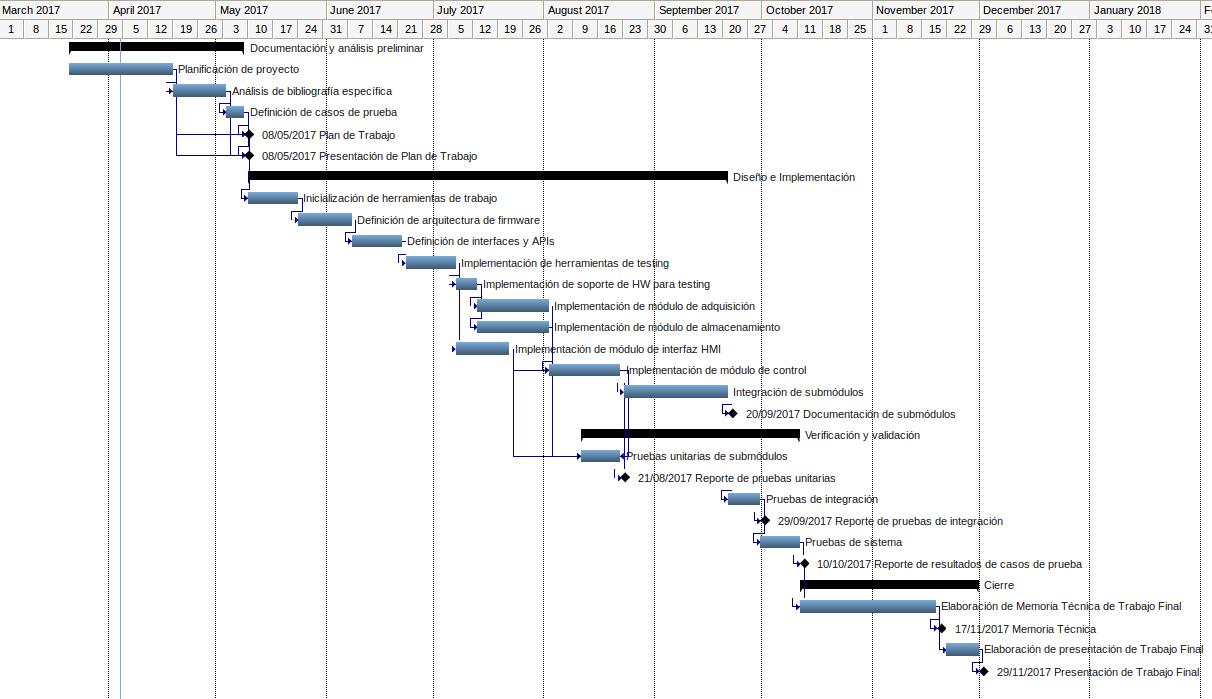
\includegraphics[height=.85\textheight]{./Figuras/Gantt-2.png}
\caption{Ejemplo de diagrama de Gantt rotado}
\label{fig:diagGantt}
\end{figure}

\end{landscape}

\end{consigna}


\section{12. Presupuesto detallado del proyecto}
\label{sec:presupuesto}

\begin{consigna}{red}
Si el proyecto es complejo entonces separarlo en partes:
\begin{itemize}
	\item Un total global, indicando el subtotal acumulado por cada una de las áreas.
	\item El desglose detallado del subtotal de cada una de las áreas.
\end{itemize}

IMPORTANTE: No olvidarse de considerar los COSTOS INDIRECTOS.

\end{consigna}

\begin{table}[htpb]
\centering
\begin{tabularx}{\linewidth}{@{}|X|c|r|r|@{}}
\hline
\rowcolor[HTML]{C0C0C0} 
\multicolumn{4}{|c|}{\cellcolor[HTML]{C0C0C0}COSTOS DIRECTOS} \\ \hline
\rowcolor[HTML]{C0C0C0} 
Descripción &
  \multicolumn{1}{c|}{\cellcolor[HTML]{C0C0C0}Cantidad} &
  \multicolumn{1}{c|}{\cellcolor[HTML]{C0C0C0}Valor unitario} &
  \multicolumn{1}{c|}{\cellcolor[HTML]{C0C0C0}Valor total} \\ \hline
 &
  \multicolumn{1}{c|}{} &
  \multicolumn{1}{c|}{} &
  \multicolumn{1}{c|}{} \\ \hline
 &
  \multicolumn{1}{c|}{} &
  \multicolumn{1}{c|}{} &
  \multicolumn{1}{c|}{} \\ \hline
\multicolumn{1}{|l|}{} &
   &
   &
   \\ \hline
\multicolumn{1}{|l|}{} &
   &
   &
   \\ \hline
\multicolumn{3}{|c|}{SUBTOTAL} &
  \multicolumn{1}{c|}{} \\ \hline
\rowcolor[HTML]{C0C0C0} 
\multicolumn{4}{|c|}{\cellcolor[HTML]{C0C0C0}COSTOS INDIRECTOS} \\ \hline
\rowcolor[HTML]{C0C0C0} 
Descripción &
  \multicolumn{1}{c|}{\cellcolor[HTML]{C0C0C0}Cantidad} &
  \multicolumn{1}{c|}{\cellcolor[HTML]{C0C0C0}Valor unitario} &
  \multicolumn{1}{c|}{\cellcolor[HTML]{C0C0C0}Valor total} \\ \hline
\multicolumn{1}{|l|}{} &
   &
   &
   \\ \hline
\multicolumn{1}{|l|}{} &
   &
   &
   \\ \hline
\multicolumn{1}{|l|}{} &
   &
   &
   \\ \hline
\multicolumn{3}{|c|}{SUBTOTAL} &
  \multicolumn{1}{c|}{} \\ \hline
\rowcolor[HTML]{C0C0C0}
\multicolumn{3}{|c|}{TOTAL} &
   \\ \hline
\end{tabularx}%
\end{table}


\section{13. Gestión de riesgos}
\label{sec:riesgos}

\begin{consigna}{red}
a) Identificación de los riesgos (al menos cinco) y estimación de sus consecuencias:
 
Riesgo 1: detallar el riesgo (riesgo es algo que si ocurre altera los planes previstos de forma negativa)
\begin{itemize}
	\item Severidad (S): mientras más severo, más alto es el número (usar números del 1 al 10).\\
	Justificar el motivo por el cual se asigna determinado número de severidad (S).
	\item Probabilidad de ocurrencia (O): mientras más probable, más alto es el número (usar del 1 al 10).\\
	Justificar el motivo por el cual se asigna determinado número de (O). 
\end{itemize}   

Riesgo 2:
\begin{itemize}
	\item Severidad (S): 
	\item Ocurrencia (O):
\end{itemize}

Riesgo 3:
\begin{itemize}
	\item Severidad (S): 
	\item Ocurrencia (O):
\end{itemize}


b) Tabla de gestión de riesgos:      (El RPN se calcula como RPN=SxO)

\begin{table}[htpb]
\centering
\begin{tabularx}{\linewidth}{@{}|X|c|c|c|c|c|c|@{}}
\hline
\rowcolor[HTML]{C0C0C0} 
Riesgo & S & O & RPN & S* & O* & RPN* \\ \hline
       &   &   &     &    &    &      \\ \hline
       &   &   &     &    &    &      \\ \hline
       &   &   &     &    &    &      \\ \hline
       &   &   &     &    &    &      \\ \hline
       &   &   &     &    &    &      \\ \hline
\end{tabularx}%
\end{table}

Criterio adoptado: 
Se tomarán medidas de mitigación en los riesgos cuyos números de RPN sean mayores a...

Nota: los valores marcados con (*) en la tabla corresponden luego de haber aplicado la mitigación.

c) Plan de mitigación de los riesgos que originalmente excedían el RPN máximo establecido:
 
Riesgo 1: plan de mitigación (si por el RPN fuera necesario elaborar un plan de mitigación).
  Nueva asignación de S y O, con su respectiva justificación:
  - Severidad (S): mientras más severo, más alto es el número (usar números del 1 al 10).
          Justificar el motivo por el cual se asigna determinado número de severidad (S).
  - Probabilidad de ocurrencia (O): mientras más probable, más alto es el número (usar del 1 al 10).
          Justificar el motivo por el cual se asigna determinado número de (O).

Riesgo 2: plan de mitigación (si por el RPN fuera necesario elaborar un plan de mitigación).
 
Riesgo 3: plan de mitigación (si por el RPN fuera necesario elaborar un plan de mitigación).

\end{consigna}


\section{14. Gestión de la calidad}
\label{sec:calidad}

\begin{consigna}{red}
Elija al menos diez requerientos que a su criterio sean los más importantes/críticos/que aportan más valor y para cada uno de ellos indique las acciones de verificación y validación que permitan asegurar su cumplimiento.

\begin{itemize} 
\item Req \#1: copiar acá el requerimiento.

\begin{itemize}
	\item Verificación para confirmar si se cumplió con lo requerido antes de mostrar el sistema al cliente. Detallar 
	\item Validación con el cliente para confirmar que está de acuerdo en que se cumplió con lo requerido. Detallar  
\end{itemize}

\end{itemize}

Tener en cuenta que en este contexto se pueden mencionar simulaciones, cálculos, revisión de hojas de datos, consulta con expertos, mediciones, etc.  Las acciones de verificación suelen considerar al entregable como ``caja blanca'', es decir se conoce en profundidad su funcionamiento interno.  En cambio, las acciones de validación suelen considerar al entregable como ``caja negra'', es decir, que no se conocen los detalles de su funcionamiento interno.

\end{consigna}

\section{15. Procesos de cierre}    
\label{sec:cierre}

\begin{consigna}{red}
Establecer las pautas de trabajo para realizar una reunión final de evaluación del proyecto, tal que contemple las siguientes actividades:

\begin{itemize}
	\item Pautas de trabajo que se seguirán para analizar si se respetó el Plan de Proyecto original:
	 - Indicar quién se ocupará de hacer esto y cuál será el procedimiento a aplicar. 
	\item Identificación de las técnicas y procedimientos útiles e inútiles que se emplearon, y los problemas que surgieron y cómo se solucionaron:
	 - Indicar quién se ocupará de hacer esto y cuál será el procedimiento para dejar registro.
	\item Indicar quién organizará el acto de agradecimiento a todos los interesados, y en especial al equipo de trabajo y colaboradores:
	  - Indicar esto y quién financiará los gastos correspondientes.
\end{itemize}

\end{consigna}


\end{document}
